\section{Evaluation}

We compare our approach with the scaled versions of group fairness \cite{Zhao2017MenAL} and \cite{Beutel2017DataDA} for subgroups. In \cite{Zhao2017MenAL}, Zhao, et al. optimize for overall accuracy in the constrained setting of ensuring equal false positive rates, but is generally applicable to other measures of performance. For our comparison we implement a Lagrangian relaxation which adds penalty for each subgroup that deviates from the overall accuracy. In \cite{Beutel2017DataDA}, Beutel et al, they implement bias mitigation as a way of forgetting the sensitive group membership by back-propagating negative gradients in a multi headed feedforward neural network. We scale the same for subgroups defined over multiple sensitive variables, where the auxiliary head aims to predict the subgroup class (multi-class classification instead of binary).

\subsection{Synthetic Data}
We perform the comparison for both synthetic toy data with the setup similar to the use case mentioned in the above section and the UCI Census Adult dataset where based on demographic information, the task is to predict the income category. The sensitive variables considered in this task are gender and race.

Table \ref{tab:synthetic_subgroups} shows that for many of the synthetic cases where it is possible for all subgroups to achieve same level of accuracy, we see that our approach remains similar in subgroup performance \cite{Zhao2017MenAL} and \cite{Beutel2017DataDA}. However, for the use case where some subgroups differ in their "optimal" performance, \cite{Zhao2017MenAL} fails to achieve the "optimal" accuracy for all subgroups and hence results in lower overall accuracy. \cite{Beutel2017DataDA} however continues to perform equally well, similar to our approach in these scenarios.

\begin{table}[tp]
\footnotesize

\caption{UCI Adult dataset with bias mitigation algorithms}
\begin{center}
\begin{tabular}{lccccc}
\hline
\textbf{Model} & \textbf{Accuracy} & \textbf{FPR} & \textbf{FNR} & \textbf{Discrepancy} & \textbf{Pareto Loss}\\\hline
Baseline (no bias loss) & 0.630 & 0.253 & 0.747 & 0.199 & 0.016\\
Minimize Discrepancy & 0.619 & 0.283 & \textbf{0.712} & \textbf{0.167} & 0.133\\
Adversarial Loss & 0.648 & 0.224 & 0.769 & 0.226 & 0.077\\
Pareto-Efficient Loss & \textbf{0.678} & \textbf{0.165} & 0.830 & 0.250 & \textbf{0.000}\\\hline
\end{tabular}
\end{center}
\label{tab:uci_comparison}
\normalsize
\end{table}%

\begin{table}[tp]
\footnotesize
\caption{Change in overall accuracy as compared to baseline on synthetic dataset}
\begin{center}
\begin{tabular}{lccc}
\hline
\textbf{\vtop{\hbox{Confounding dependency}\hbox{Mean of normal distribution}}} & \textbf{Pareto} & \textbf{Minimize Discrepancy} & \textbf{Adversarial}\\\hline
2*a + 1*b & 0 & 0 & 0\\
2*b - 2*a & 0 & 0.02 & 0.02\\
4*b & 0 & 0 & -0.002\\
8*b & 0 & -0.06 & 0\\
2*a + 2*b + 2*d & 0 & 0 & 0\\
\vtop{\hbox{\strut (a,b): \{(0,0): 3, (0,1): 11,}\hbox{\strut (1,0): 4, (1,1): 8\}}}
 & 0 & 0 & 0\\
\vtop{\hbox{\strut (a,b): \{(0,0): 3, (0,1): 1,}\hbox{\strut (1,0): 4, (1,1): 8\}}}
 & 0 & -0.04 & -0.04\\
\vtop{\hbox{\strut (a,b): \{(0,0): 3, (0,1): 11,}\hbox{\strut (1,0): 4, (1,1): 9\}}}
 & 0 & -0.01 & -0.01\\
\vtop{\hbox{\strut (a,b): \{(0,0): 3, (0,1): 11,}\hbox{\strut (1,0): 4, (1,1): 9\}}\hbox{Prevalence ratio: 1:9:1:9}}
 & 0 & \textbf{-0.1} & 0\\\hline
\end{tabular}
\end{center}
\label{tab:synthetic_subgroups}
\normalsize
\end{table}%

\subsection{UCI Census Data}
Table \ref{tab:uci_comparison} shows that for the UCI Census Adult dataset, \cite{Zhao2017MenAL} performs significantly well in terms of lowering the discrepancy of the subgroup's accuracy from the overall accuracy (measured in discrepancy). This is expected as per the objective that \cite{Zhao2017MenAL} set out to achieve. \cite{Beutel2017DataDA} achieves similar, but comparatively worse and our approach performs the worst as compared to the baseline which did not have any bias mitigation. However, the scenario is different when considering the Pareto Loss, i.e the penalty that each subgroup deviates from the optimal of the respective subgroup. We see that our approach achieves zero Pareto-Loss, while \cite{Zhao2017MenAL} and \cite{Beutel2017DataDA} have significant Pareto losses. Table \ref{tab:uci_subgroups} clarifies why this is the case, where we see that each of the subgroups have better accuracy, some even better than the baseline than all the other approaches. This again, is evident from the objective function which we set out to achieve, where each group is trying to achieve their heuristic optimal performance (quoted in the last row of Table \ref{tab:uci_subgroups}).

\begin{table}[tp]
\footnotesize
\caption{Subgroup performance on UCI Adult dataset}
\begin{center}
\begin{tabular}{lccccc}
\hline
\textbf{Model} & \textbf{Subgroup 1} & \textbf{2} & \textbf{3} & \textbf{4} & \textbf{Pareto Loss}\\\hline
Baseline (no bias loss) & 0.890 & 0.883 & 0.818 & 0.784 & 0.016\\
Minimize Discrepancy & 0.853 & 0.856 & 0.806 & 0.778 & 0.133\\
Adversarial Loss & 0.882 & 0.872 & 0.824 & 0.780 & 0.077\\
Pareto-Efficient Loss & \textbf{0.935} & \textbf{0.915} & \textbf{0.844} & \textbf{0.797} & \textbf{0.000}\\
Subgroup Pareto Frontier & 0.934 & 0.894 & 0.815 & 0.783 & N/A \\\hline
\end{tabular}
\end{center}
\label{tab:uci_subgroups}
\normalsize
\end{table}%

\subsection{Effect of Model capacity}
We used 3 layers of feed forward networks with 256, 128 and 64 neurons fully connected in all our comparisons of relevant losses. However, we did notice that the difference in the losses varied with the size of the model used as noted in Table \ref{tab:uci_model_size}. The gains achieved from Pareto loss is higher when the model capacity increases, as it is able to capture the per subgroup specific performance updates with more number of parameters.

\begin{table}[tp]
\footnotesize
\caption{Effect of model size on subgroup performance (compared with baseline) on UCI Adult dataset}
\begin{center}
\begin{tabular}{lcccc}
\hline
\textbf{Model size} & \textbf{Subgroup 1} & \textbf{2} & \textbf{3} & \textbf{4}\\\hline
64 & 0.923 (0.929) & 0.898 (0.914) & 0.812 (0.849) & 0.733 (0.809)\\
$128,64$ & 0.902 (0.925) & 0.884 (0.909) & 0.820 (0.849) & 0.781 (0.805)\\
$256,128,64$ & \textbf{0.935} (0.890) & \textbf{0.915} (0.883) & \textbf{0.844} (0.818) & \textbf{0.797} (0.784)\\\hline
\end{tabular}
\end{center}
\label{tab:uci_model_size}
\normalsize
\end{table}%


\subsection{Confounding Variable Detection}
To detect the potential confounding variables in the UCI Census dataset, we first ran the baseline logistic regression model to predict income bracket, without the sensitive variables: race and gender. We then evaluated the performance of each of the subgroups when conditioned on values of each of the other feature variables to calculate the subgroup discrepancy for each variable. If the subgroup discrepancy conditioned on a feature is less than a upper threshold,  $\alpha$, then we might define those features as potential resolving variables. So potentially, within a bound of discrepancy  $\alpha$, we can explain away all the subgroups discrepancy by conditioning on such features. Similarly, if the subgroup discrepancy when conditioned on a features is more than a lower threshold $\beta$, such variables are defined as unresolving variables and expose the discrepancy within the subgroups. For continuous variables such as education, we quantize the values into 10 levels and plot their discrepancy as shown in Figure \ref{edu_disc}. Potential confounding variables can also be easily compared quantitatively using the lower and upper thresholds for subgroup discrepancy as shown in Figure \ref{all_disc}.

\begin{figure}[htbp]
	\begin{center}
		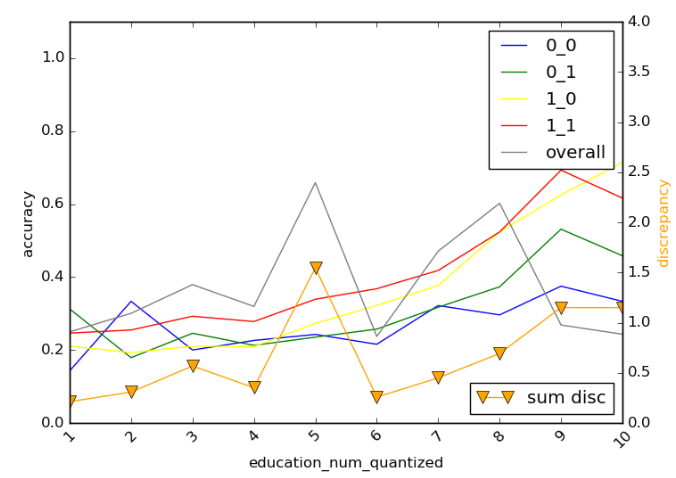
\includegraphics[width=3.2in,height=1.6in]{education_disc.png} 
        \setlength{\belowcaptionskip}{-8pt} 
		\caption{Education as a potential confounding variable in the UCI Census dataset($\alpha=1.6, \beta=0.2$)}
		\label{edu_disc}
	\end{center}
\end{figure}

\begin{figure*}[htbp]
\centering  
\subfigure[Hours per week ($\alpha=1.1, \beta=0.1$)]{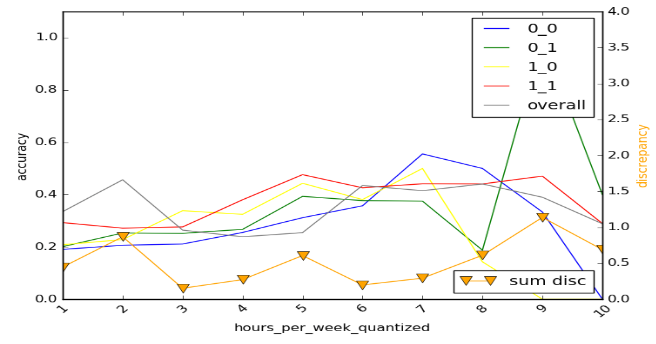
\includegraphics[width=0.45\linewidth]{age_disc}}
\subfigure[Occupation ($\alpha=2.0, \beta=0.05$)]{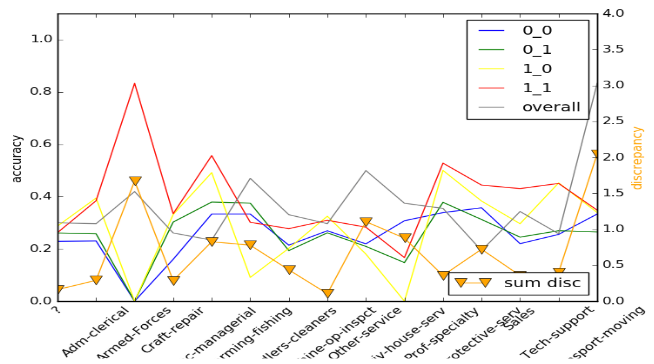
\includegraphics[width=0.45\linewidth]{occupation_disc}}
\subfigure[Relationship ($\alpha=0.9, \beta=0.1$)]{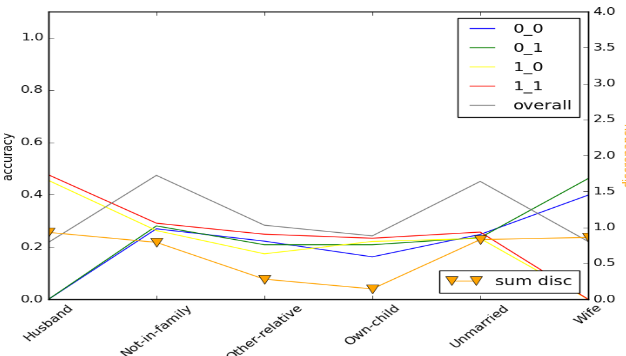
\includegraphics[width=0.45\linewidth]{relation_disc}}
\subfigure[Age ($\alpha=1.5, \beta=0.01$)]{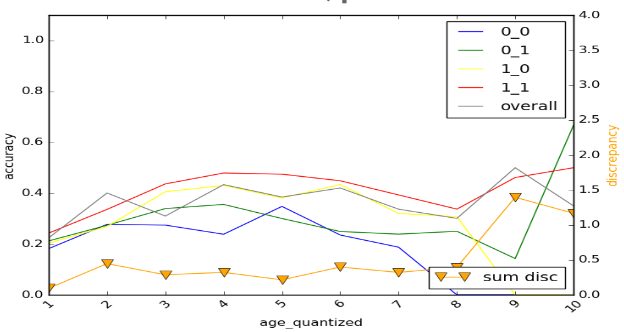
\includegraphics[width=0.45\linewidth]{age_q_disc}}
\caption{Potential confounding variables in UCI Census dataset with their corresponding thresholds of discrepancy}
\label{all_disc}
\end{figure*}



\subsection{Summary of Results}
	In this paper we sought to establish several points, in the application of sensitive variable constraints in the spirit of fairness for  machine learning models. 
\begin{enumerate}
	\item \textbf{Influence of Confounding Factors} - In order to perform a macro analysis of the trade-offs in fairness, possible confounding factors in relation to sensitive variables need to identified.  Without apriori knowledge of causality, a statistical analysis can only hypothesis variable effect.  In this paper, we suggest a standard for identifying possible confounding variables in relation to pre-defined sensitive variables. Similarly, we suggest incorporating the possible confounding variables into the sensitive variable subgroup constraints to mitigate their effects.  \par
    	In essence this approach is examining the individual conditional posterior probabilities for each subgroup.  The authors acknowledge that this approach will grow exponentially with the number of sensitive variables and possible confounding variables. As such this solution is only appropriate for a limited number of sensitive variables within a dataset. \par
    
    \item \textbf{Evaluate Subgroups Individually} - When more than one sensitive variable is present, evaluating subgroups individually and predicated on possible confounding factors mitigates the effects of prevalence on a dataset.  In real world problems, the population of subgroups with combinations of sensitive variables is unlikely to be equivalent and often skewed to a dominant sub-population. Similarly when sample populations are heavily skewed in prevalence, metrics such as accuracy can be deceptive and entirely mis-categorize a minority subgroup. In enforcing sensitive variable constraints, the authors are motivated to apply such Lagrangian constraints to individually to BOTH the False Positive and False Negative Loss functions for each subgroup.  
    
    \item \textbf{Dynamic Subgroup Fairness Constraints}  - The paper attempted to identify several instances where fixed accuracy constraints for individual subpopulations, even with a relaxation parameters, would be inappropriate for real-world datasets. In fact, fixed constraints may perform sub-optimally increasing inequity. The paper offers a Pareo-Efficient algorithm and methodology to address this scenario. As dissected in Menon et. al \cite{Menon2018TheCO}, there will be a degradation in performance due to a fairness constraint unless the existing subgroup populations have equivalent possible sample accuracies. The algorithm in this paper, using an optimal heuristic derived either from experiments with the existing data or another method such as transfer learning, mitigates the cited global(macro) and subgroup(micro) performance degradation.  As demonstrated in Table \ref{tab:uci_subgroups}, the accuracy for each subgroup  in the UCI dataset is noticeably improved with the paper's Pareto-Efficient Loss methodology. Similarly the global accuracy is improved. 
 \end{enumerate}
   
 
 
 
 
 
    

    
